\documentclass[landscape,a0b]{a0poster}
%\documentclass[letterpaper,10pt]{article}

\usepackage[utf8]{inputenc}
%\usepackage{kpfonts}
\usepackage[top=1in, bottom=1in, left=1in, right=1in]{geometry}
\usepackage{parskip}
\usepackage{tabularx}
\usepackage{qtree}
\usepackage{graphicx}
\usepackage{xfrac}
\usepackage{forest}
\usepackage{tikz-dependency}
\usepackage{graphicx}
\usepackage{float}
\usepackage{amsmath}
\usepackage{varioref}
\usepackage{hyperref}
\usepackage{xfrac}
\usepackage{amsmath}
\usepackage{bm}
\usepackage{pgfplots}
\usepackage{pbox}
\usepackage{framed}
\usepackage[authordate,bibencoding=auto,strict,backend=biber,natbib]{biblatex-chicago}
\usepackage{comment}
\usepackage{enumitem}
\usepackage{float}
\usepackage{dblfloatfix}
\usepackage{afterpage}
\usepackage{multirow}
\usepackage{multicol}
\usepackage[compact]{titlesec}

\renewcommand{\cite}{\citep}
\numberwithin{equation}{section}
\renewcommand{\tabularxcolumn}[1]{>{\small}m{#1}}

\def\topfraction{0.9} % 90 percent of the page may be used by floats on top
\def\bottomfraction{0.9} % the same at the bottom
\def\textfraction{0.01}

\DeclareMathOperator*{\argmin}{arg\,min}
\DeclareMathOperator*{\argmax}{arg\,max}

% http://tex.stackexchange.com/a/33547
\newcommand{\approptoinn}[2]{\mathrel{\vcenter{
  \offinterlineskip\halign{\hfil$##$\cr
    #1\propto\cr\noalign{\kern2pt}#1\sim\cr\noalign{\kern-2pt}}}}}

\newcommand{\appropto}{\mathpalette\approptoinn\relax}

\addbibresource{prop.bib}

%opening
\title{\Huge Incrementally Identifying Objects from Referring Expressions using Spatial Object Models}
\author{Gaurav Manek, Stefanie Tellex \\ Humans to Robots Laboratory, Brown University \\ \texttt{gaurav\_manek@brown.edu, stefie10@cs.brown.edu}}
\date{}
\begin{document}

\setlength{\columnsep}{1in}
\begin{multicols*}{3}
[
\maketitle
]

\titlespacing*{\section}{0pt}{0pt}{7pt}
\thispagestyle{empty}

\begin{framed}
\section{Abstract}
An important problem in human-robot interaction is that of referring expressions: phrases used to identify a particular object among others. Existing parsing models all operate on entire sentences. Incrementally parsing referring expressions is important for human-robot interaction and conversational feedback. We present a model for parsing real-word referring expressions, trained and tested on human-provided data. In our test corpus, when presented with the entire sentence, our model ranks the correct object as the most likely 60.3\% of the time, and ranks the correct object in the top three 79.0\% of the time. Given the entire sentence humans identify the correct object 79.0\% of the time. With 50\%, 80\% and 90\% of the sentence, the model ranks the correct object as the most likely 17.4\%, 27.8\%, and 36.2\% of the time. Our parser is capable of keeping up with human speech, with 80\% of all words processed on commodity hardware within 10ms, and 95\% of all words in about 300ms.

\end{framed}

\titlespacing*{\section}{0pt}{14pt plus 4pt}{0.7ex minus .2ex}


\section{Introduction}

Referring expressions are phrases used to identify a particular object in a scene by describing it and its relative position to other objects. The integration of \emph{social feedback}, where the robot shows its understanding of a human's utterances by generating small responses as it listens to the human, can prompt clarifications from the human and improve the accuracy of referring expression parsing in interactive contexts. However, this requires robots to be able to parse the human input \emph{incrementally}: updating its understanding as each next word is uttered. In this paper we present an incremental referring expression parser that can process prepositional phrases. 

\section{Example}

\newcommand{\inctest}[1]{\includegraphics[trim={0 3cm 5cm 3.5cm},clip,width=0.15\textwidth]{test_set_example/Slide#1}}
\newcolumntype{L}{>{\centering\arraybackslash}m{0.15\textwidth}}
\begin{tabular}{LL}
\inctest{5} & \inctest{6} \\
   ~
& \emph{``--''} \\
  Cube 4 is the target of the referring expression. 
& Without any information, distribution is uniform over all objects. \\[2em]
\inctest{7} & \inctest{9} \\
  \emph{``Orange--''}
& \emph{``Orange cube between--''} \\
  The first word makes many objects very unlikely.
& Symmetry of the distribution is broken by the preposition. \\[2em]
\inctest{11} & \inctest{15} \\
  \emph{``Orange cube between the toy--''}
& \emph{``Orange cube between the toy and the tape roll.''} \\
  Providing a grounding further changes the distribution. 
& Cube 4 has the highest assigned probability.
\end{tabular}
\begin{center}
\textit{Figure 1: Example}
\end{center}
~

\section{Technical Approach}

\begin{tabularx}{0.3\textwidth}{@{} >{\hsize=.5\hsize \centering}X >{\hsize=.45\hsize}X @{}} 
\multicolumn{2}{c}{``The orange cube between the red thing and the yellow thing.''} \\ 
\multicolumn{2}{c}{$\Downarrow$} \\ 
% Chunking	
\begin{tabular}{c}
$\underbrace{\text{The orange cube}}_{\texttt{SNP}}$
$\underbrace{\text{between}}_{\texttt{PRP}}$
$\underbrace{\text{the red thing}}_{\texttt{SNP}}$
\\
$\underbrace{\text{and}}_{\texttt{PRP}}$
$\underbrace{\text{the yellow thing}}_{\texttt{SNP}}$
$\underbrace{\text{.}}_{\texttt{.}}$
\end{tabular}
& 
\textbf{Chunking}

First, we use Mallet, \citep{McCallumMALLET} a sequence tagging library, to tag the referring expression with a set of tags. The tags were developed to suit our use case, and are a simplification of the typical English parts-of-speech tags.

\\ $\Downarrow$ \\[0.2cm] 

\scalebox{.9}{\Tree [.TARGET \qroof{The orange cube}.OBJECT [.BETWEEN   \qroof{the red thing}.OBJECT \qroof{the yellow thing}.OBJECT ] ]} &

\textbf{Semantic Tree}

The tagged sequence is then converted to a semantic tree. Because of the simplified tag set in the previous step, this transformation is deterministic.

\\ $\Downarrow$ \\[0.2cm] 

\scalebox{.9}{\Tree [.TARGET \qroof{$\{\sfrac{1}{16}, \sfrac{1}{16}, \ldots, \sfrac{1}{16}\}$}.OBJECT [.BETWEEN   \qroof{$\{0, \sfrac{1}{8}, \ldots, 0\}$}.OBJECT \qroof{$\{0, 0, \ldots, \sfrac{1}{2}\}$}.OBJECT ] ]} 

~

\scriptsize{\{\textit{orange\_1}, \textit{red\_1}, $\ldots $, \textit{yellow\_2}\}}

&
\textbf{Language Model}

We use a language model to convert each of the simple noun phrases into individual distributions over possible objects.

\\ $\Downarrow$ & ~ \\[0.2cm] 

\scalebox{.9}{\Tree [.TARGET \qroof{$\{90\%, 2\%, \ldots 1\%\}$}.OBJECT ]} 

~

\scriptsize{\{\textit{orange\_1}, \textit{orange\_2}, $\ldots $, \textit{blue\_1}\} }

&
\textbf{Bottom-up Evaluation}

We evaluate the tree from the bottom upwards, using spatial features and trained weights to convert each input distribution and the type of preposition into a set of output scores. The final result is the object with the highest score.
\end{tabularx}


\begin{center}
\textit{Figure 2: Technical Approach}
\end{center}



\section{Evaluation} 

We collected a corpus of human-generated data using Human Intelligence Tasks (HITs) on the Amazon Mechanical Turk (AMT) platform and 19 hand-generated scenes, of which 10 were reserved for the test set. Scenes were similar to the example in Figure 1.  For each orange cube in each scene, 9 different workers produced  referring expressions and each expression was further evaluated by three separate human raters. 

\begin{center}
  \begin{tabular}{| r r | c | c | c || c c |} \hline
     & & \multicolumn{5}{c|}{Rate of correct identification, Test (\%)} \\
     & & \multicolumn{3}{c||}{Baselines} & \multicolumn{2}{c|}{Results} \\
     \multicolumn{2}{|c|}{Preposition}
			                      &   Human & Unigram & Random &  Top-1 & Top-3 \\\hline
26.8\% & \textit{between}       & 88.2  & 14.3  & 7.1   & 77.5  & 97.1 \\
21.3\% & \textit{near}          & 82.5  & 17.2  & 7.3   & 64.7  & 88.1 \\
14.2\% & \textit{behind}        & 76.9  & 15.7  & 6.9   & 81.5  & 94.4 \\
11.0\% & \textit{in front of}   & 69.9  & 17.9  & 7.5   & 57.1  & 88.1 \\
9.4\% & \textit{left of}        & 89.8  & 16.1  & 7.3   & 69.4  & 100.0 \\
5.8\% & \textit{right of}       & 58.0  & 15.4  & 7.3   & 55.2  & 91.6 \\\hline\hline
    \multicolumn{2}{|r|}{Total} & 79.0  & 16.1  & 7.2   & 60.3  & 79.0 \\\hline
  \end{tabular}
  
\textit{Figure 3: Results}
\end{center}

Figure~3 shows the correctness rate of our algorithm when run on complete sentences, and of three baselines for comparison. The percentage next to each preposition is the fraction of sentences in the test set that contain this preposition, and so will not add up to 100\%. The baselines are:
\begin{enumerate}[topsep=0pt,itemsep=-1ex,partopsep=1ex,parsep=1ex]
	\item The \emph{Human} baseline, which was established by having humans select the object best identified by the referring expression, and scoring them against our corpus.
	\item The \emph{Unigram} baseline, which is the expectation of selecting the correct object using a simple unigram object model across the entire input sentence.
	\item The \emph{Random} baseline, the expectation of selecting the correct object by selecting one at random.
\end{enumerate}

The \emph{Results} column lists the rate of correct identification using the entire sentence as input, the \emph{Top-1} column lists the rate at which the correct object is rated the most likely by the algorithm, and the \emph{Top-3} column lists the rate at which the correct object is in the top 3 items. Should there be a tie, the rate is divided by the number of items of equal probability.

\subsection{Incremental Performance}

To evaluate the performance of the incremental algorithm, we report correctness on the test set as a fraction of each sentence in Figure~4.

Three separate lines are drawn to show the distribution of the rank of the correct option. Each Top-$k$ line includes an example if the target object has at least as much probability as the $k^\text{th}$-highest probability in the distribution. Should there be a tie, the rate is divided by the number of items of equal probability.


\begin{center}
  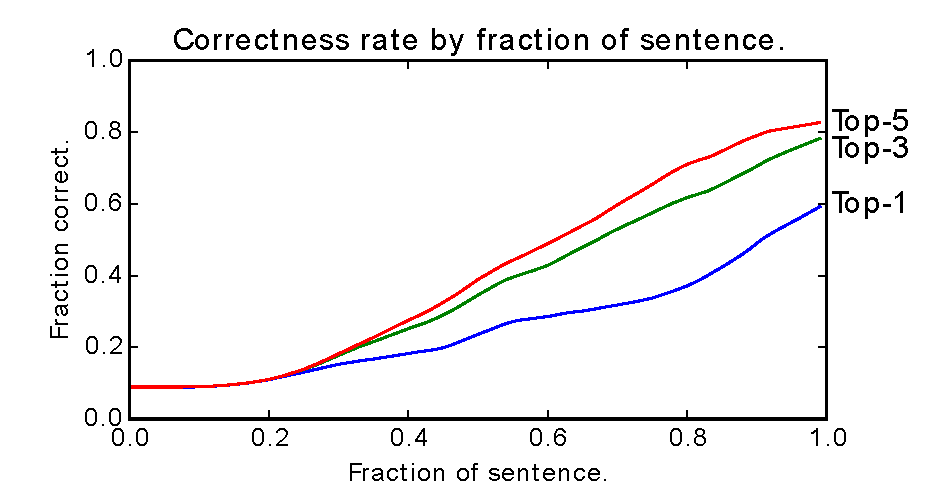
\includegraphics[width=0.45\columnwidth]{eval/cdf_by_fraction}
  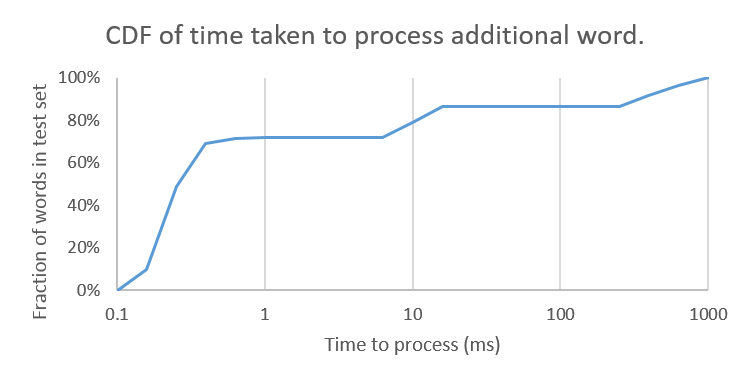
\includegraphics[width=0.45\columnwidth]{time_inc}
  
  \textit{Figure 4: Performance and time taken on test set.}
\end{center}

We also measure the amount of time our implementation takes to process each word on commodity hardware, and we compute the observed cumulative density function. As can be seen in the right chart in Figure 4, 70\% of all words are processed within 1ms, and 90\% within 300ms -- quick enough to keep up with human speech.


\section{Conclusion}
In this paper we have presented an incremental referring expression parser that can process prepositional phrases. The incremental nature of the parser is the key contribution: state-of-the-art parsers all operate on complete referring expressions. The primary future task is to integrate this with the social feedback framework on Baxter in the H2R lab and conduct user studies to investigate if this provides a measurable improvement to user interaction.

\section{Related Work}

Prepositional phrases have not been subject to as much computational analysis and study as noun- and verb-phrases. The current research on the topic uses referring expressions as parts of larger phrases, such as commands. There is an existing family of related work by \citet{tellex2011understanding}, \citet{UW_RSE_ICML2012}, and \citet{artzi2013weakly}, all of whom present modern models to process referring expressions. These models all operate on entire input sentences and are designed to parse general instructions and commands instead of only prepositional phrases. 
\citet{tellex2011understanding} present the $G^3$ framework. We use several key ideas from this paper: in particular we implicitly assume the binary correspondence variable that their model maximizes. Our algorithm is inspired in part by the algorithm they present.


\section{Selected References}
\nocite{artzi2013weakly}
\nocite{tellex2011understanding}
\nocite{UW_RSE_ICML2012}


\printbibliography[heading=none]

\end{multicols*}

\end{document}
